\documentclass[a4paper,landscape]{article}
\usepackage[english]{babel}
\usepackage[top=2cm,bottom=2cm,left=1cm,right=1cm,marginparwidth=1.75cm]{geometry}\usepackage{amsmath}
\usepackage{tikz}
\usetikzlibrary{shapes}
\usetikzlibrary{plotmarks}
\usepackage[colorlinks=true, allcolors=blue]{hyperref}
\usetikzlibrary{positioning}
\usetikzlibrary{shapes.geometric}
\begin{document}
\definecolor{zx_red}{RGB}{253, 160, 162}
\definecolor{zx_green}{RGB}{206, 254, 206}
\definecolor{hedgeColor}{RGB}{40, 160, 240}
\definecolor{phaseColor}{RGB}{14, 39, 100}
\scalebox{3.000000}{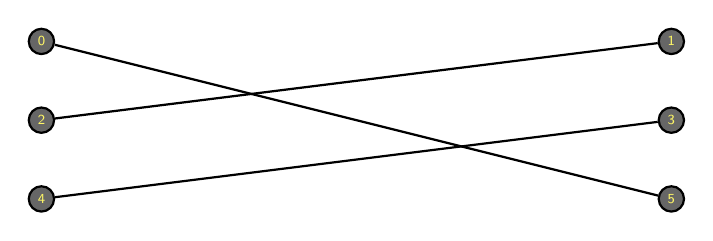
\begin{tikzpicture}[
font = \sffamily,
	 yscale=-1,
	 boun/.style={circle, text=yellow!60, font=\sffamily, draw=black!100, fill=black!60, thick, text width=3mm, align=center, inner sep=0pt},
	 hbox/.style={regular polygon, regular polygon sides=4, font=\sffamily, draw=yellow!40!black!100, fill=yellow!40, text width=2.5mm, align=center, inner sep=0pt},
	 zspi/.style={circle, font=\sffamily, draw=green!60!black!100, fill=zx_green, text width=5mm, align=center, inner sep=0pt},
	 xspi/.style={circle, font=\sffamily, draw=red!60!black!100, fill=zx_red, text width=5mm, align=center, inner sep=0pt},
	 hedg/.style={draw=hedgeColor, thick},
	 sedg/.style={draw=black, thick},
];
    % Vertices
    \node[boun](0)  at (0.000000,0) {{\tiny 0}};
    \node[boun](1)  at (8.000000,0) {{\tiny 1}};
    \node[boun](2)  at (0.000000,1) {{\tiny 2}};
    \node[boun](3)  at (8.000000,1) {{\tiny 3}};
    \node[boun](4)  at (0.000000,2) {{\tiny 4}};
    \node[boun](5)  at (8.000000,2) {{\tiny 5}};
    % Edges
    \draw[sedg] (0) -- (5);
    \draw[sedg] (1) -- (2);
    \draw[sedg] (3) -- (4);
\end{tikzpicture}}
\end{document}
